\documentclass{standalone}
\usepackage{tikz-qtree}
\usepackage{fontspec}
    \setmainfont{Charis SIL}
\begin{document}
% In the preamble:

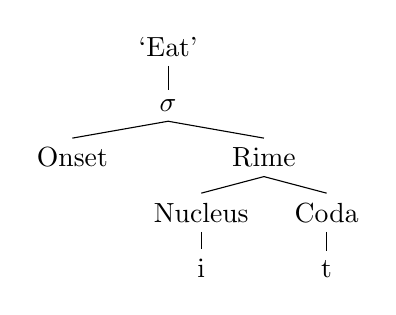
\begin{tikzpicture}[sibling
distance=10pt, level distance=20pt]
\tikzset{frontier/.style={distance from root=80pt}}
\Tree[.`Eat'
     [.$\sigma$ [.Onset  ] [.Rime [.Nucleus i ] [.Coda t ] ] ] ]
         
\end{tikzpicture}

\end{document}
